% SLOGANS: 
% - Chapter-specific: \"dynamic discreteness\" and \"real gradience\" (twin themes)
% - Book-wide: \"categories are real because they're maintained\" appears in conclusion
% See notes/book-slogans.md for the slogan strategy.

\chapter{Discrete from continuous}
\label{ch:dynamic-discreteness}

% Chapter 4 introduces HPC framework; this chapter applies it to the discreteness problem.

Thursday, 4 December 2025 was one of the most intellectually exciting days of my life.

I had conceived of this book~-- or perhaps I'd say the conceptual process had come to a head~-- the previous Saturday, when I created a project folder on my computer called \texttt{HPC book} and sent a synopsis to some friends with the subject line \enquote{Does linguistics need this book?} I've learned to treat the act of naming a folder as the weakest possible form of commitment, but it was enough to start the chain reaction.

Geoff Pullum said yes. Ryan Nefdt said yes~-- and added something I hadn't thought of:

\begin{quote}
I personally favour a phase transition approach in which discreteness really is a feature of a system under a particular kind of measurement and context and continuity under a different one (like water moving from liquid to gas takes on different properties). So borrowing more from physics than biology.
\end{quote}

I woke very early the next morning thinking about phase transitions~-- and about a paper I'd written two months earlier and then set aside. That paper had formalised Sorites tolerance using hyperreal numbers, inspired by work by Toby Ord. It had been \enquote{sitting in a drawer}, waiting for a use. Now it had one.

By bedtime that evening, I had the first draft of this chapter.

Here is the puzzle I hadn't known I needed to solve.

\section{The gradience problem}
\label{sec:5:gradience-problem}

Linguistic categories look discrete: a word is a noun or it isn't, a sentence is grammatical or it isn't, a sound is /\ipa{ɪ}/ or /\ipa{ɛ}/ in the \mention{pin}/\mention{pen} contrast for the dialects that maintain it. But the properties underlying those categories are continuous: frequency distributions shade smoothly from one pattern to another, acoustic cues vary continuously (vowel formants don't come in bins), semantic features don't come with sharp edges. How do discrete categories emerge from continuous substrates?

Both definition-based essentialism and \enquote{unreal} exemplarism fail to solve this. As argued in Chapter~\ref{ch:kinds-without-essences}, we need a view where emergent patterns maintained by reliable mechanisms constitute real kinds. We need \term{dynamic discreteness}~-- discreteness that is achieved, not given.

The answer lies in scale. A change that's negligible when you're far from a boundary becomes appreciable when you're close. That's why tolerance intuitions coexist with boundary intuitions~-- both are correct, just in different regimes. And the mechanisms that maintain categories~-- acquisition, entrenchment, alignment, transmission~-- are what keep the boundary where it is.

A note on what follows: the discreteness is predicate-by-predicate. This framework doesn't force exclusivity~-- an item can be in two basins, as with dual membership in the noun-adjective zone. The worry that \mention{fun} or \mention{near} will be squeezed into one category or the other is addressed rather than suppressed. Overlap is allowed; the question is what maintains it.

\subsection{The phase-transition intuition}
\label{subsec:5:phase-intuition}

Chapter~\ref{ch:kinds-without-essences} introduced a physical analogy: phase transitions. Water has no essence of liquidity; the same molecules constitute ice, liquid, and steam depending on temperature and pressure. The boundaries are real and sharp enough for skating or swimming, but they are maintained by dynamics, not definitions.

Phase transitions produce categorical outcomes (solid, liquid, gas) from continuous substrates (temperature, pressure). This suggests the solution: if physical systems can exhibit discrete, stable structure without essences, perhaps linguistic categories can too. We need to say precisely what it is about the dynamics that produces discreteness.

The key insight from physics is that phase boundaries are \emph{scale-sensitive}. Near a phase boundary, small changes in temperature or pressure can flip the system from one phase to another. Far from the boundary, the same small changes have no categorial effect~-- the system remains solidly in one phase. The boundary is sharp, but its sharpness is a feature of the system at a particular scale of observation. Zoom in far enough and you find molecules fluctuating; zoom out and you find stable ice or stable water. The discreteness is real, but it emerges at the macroscopic level from continuous microscopic variation. Macroscopic discreteness is measurement-indexed: phases are crisp relative to thermometers, not relative to individual molecules.

The same logic applies to vague predicates generally. Consider a heap of sand. Ten thousand grains is clearly a heap. One grain is clearly not. The boundary seems sharp~-- at some point, removing one more grain tips the collection from heap to non-heap~-- but we cannot pinpoint it. This is the Sorites paradox. Standard responses include epistemicism (the boundary is sharp but unknowable), degree theory (heaphood comes in degrees), and supervaluationism (multiple precisifications are equally acceptable). None quite captures the phase-transition intuition: that the boundary is sharp at the right scale, located in a determinate region, and maintained by dynamics rather than essences.

\subsection{Relative tolerance}
\label{subsec:5:relative-tolerance}

To make this precise, consider what \enquote{one grain doesn't matter} really means. It can't mean that removing one grain \emph{never} makes a difference~-- that would entail that even a single grain is a heap. What it means is that removing one grain doesn't matter \emph{when you have many grains}. Ten thousand minus one is still clearly a heap. Fifty minus one might not be.

The difference is relative, not absolute. Removing one grain from ten thousand is a 0.01\% change. Removing one grain from fifty is a 2\% change. The same absolute change has different significance depending on the scale.

This suggests a principle:

\begin{quote}
\textbf{Relative Tolerance:} Changes that are negligibly small \emph{relative to the current scale} preserve category membership. Changes that are appreciable relative to the current scale may not.
\end{quote}

The principle is intuitive. When you're dealing with a clear heap~-- thousands of grains~-- removing one is negligible. When you're down to borderline cases~-- dozens of grains~-- removing one is appreciable. Tolerance holds in the first regime and fails in the second. The boundary lies where negligible changes accumulate into appreciable ones.

But \enquote{negligible} and \enquote{appreciable} are themselves vague. To make the principle precise, we need a framework that can handle the distinction rigorously. This is where nonstandard analysis helps.

The next section is therefore not a philosophical aside. The formalism is designed to derive a concrete empirical prediction: that distance-to-boundary should predict judgment variance, with a characteristic functional form. If the hyperreal story is wrong, that variance signature should not appear. If the story is right, the variance pattern is not just compatible with the framework~-- it falls out of the mathematics.

\section{A formal solution}
\label{sec:5:formal-solution}

\begin{framed}
\noindent\textbf{Skip path.} The next subsection develops a formal model using hyperreal numbers. Readers who prefer to skip the mathematics can take away three points and rejoin at §\ref{sec:5:geometry-to-mechanism}:
\begin{enumerate}
    \item Tolerance is scale-sensitive: small changes are tolerated, but they accumulate.
    \item Sharp boundaries exist at thresholds we can't precisely locate.
    \item Discrete categories and gradient intuitions are compatible~-- the discreteness is in the structure, the gradience is in our access to it.
\end{enumerate}
\end{framed}

\subsection{The hyperreal formalization}
\label{subsec:5:hyperreal}

The hyperreal numbers extend the reals with \emph{infinitesimals}~-- quantities greater than $0$ but smaller than any positive real number \citep{Goldblatt1998LecturesHyperreals}. Robinson's construction is rigorous, but we do not need its details. Here infinitesimals are a modelling device for making \emph{negligible relative to the current scale} precise without stipulating an arbitrary finite cutoff. I am not claiming speakers compute with hypernaturals; the hyperreals play the role calculus plays in physics. The application to vagueness is developed fully in \citet{reynolds2025sorites}.

Here is how the framework applies to vague predicates. Let $P$ be a predicate like \textit{is a heap}, and let $\mu(x)$ be a measure of the relevant property~-- say, grain count. For successive cases $c_i$ and $c_{i+1}$ in a series, let $\Delta\mu_i = \mu(c_{i+1}) - \mu(c_i)$ be the change from one case to the next.

The Relative Tolerance principle becomes:

\begin{quote}
If $|\Delta\mu_i|/\mu(c_i)$ is infinitesimal, then $P(c_i) \leftrightarrow P(c_{i+1})$.
\end{quote}

In plain language: if the fractional change is infinitesimally small, the predicate's truth value is preserved. This captures the intuition that proportionally tiny changes don't matter, while allowing that accumulated changes can.

Now model the entire Sorites series~-- from clear heap to clear non-heap~-- as a \emph{hyperfinite chain} of $\omega$ steps, where $\omega$ is an infinite hypernatural number (Figure~\ref{fig:hyperfinite-chain}). This is a standard construction in nonstandard analysis: a sequence indexed by hypernaturals, behaving internally like a finite sequence but containing infinitely many elements from the external perspective.

\begin{figure}[t]
\centering
\includegraphics[width=0.85\textwidth]{figures/5.hyperfinite-chain.png}
\caption{The hyperfinite Sorites chain. The predicate $P$ (e.g., \emph{is a heap}) holds at every standard natural index: tolerance preserves truth across any finite portion of the series. The cutoff $K$ lies at a hypernatural index beyond all standard naturals~-- determinate within the model but not finitely specifiable.}
\label{fig:hyperfinite-chain}
\end{figure}

Within this hyperfinite chain, by the transfer principle of nonstandard analysis, any monotone sequence from $P$-true to $P$-false has a least index $K$ at which $P$ flips. This $K$ is a hypernatural~-- not a standard natural number, but a number in the extended system. And crucially, because we've stipulated that $P$ holds at all standard indices (encoding the intuition that tolerance holds throughout any finite portion of the series), $K$ must be nonstandard: infinitely large compared to any standard natural.

The picture that emerges:

\begin{itemize}
\item \textbf{Far from $K$}: The fractional change at each step is infinitesimal. Relative Tolerance applies. The predicate is preserved.
\item \textbf{Near $K$}: The fractional change is appreciable (no longer infinitesimal at this scale). Relative Tolerance is silent. The predicate can flip.
\item \textbf{At $K$}: The boundary. Sharp, determinate, located at a specific hypernatural index~-- but epistemically inaccessible because we can't finitely specify which hypernatural.
\end{itemize}

This is why the Sorites induction fails. The inductive premise~-- \enquote{if $P(c_i)$ then $P(c_{i+1})$}~-- holds only where Relative Tolerance applies, which is far from the boundary. Near the boundary, the premise is false. The chain breaks not because tolerance is non-transitive, but because tolerance doesn't apply uniformly across the entire series.

\subsection{Sharp boundaries, fuzzy appearances}
\label{subsec:5:sharp-fuzzy}

The hyperreal model maintains classical bivalent logic throughout. At every index~-- including hypernatural indices~-- the predicate is either true or false. There are no degrees of heaphood, no fuzzy membership values. The boundary is sharp.

But the boundary is also inaccessible. It lies at a hypernatural index that we can't specify using finite means. From our finite observational standpoint, we see clear heaps, clear non-heaps, and a region of uncertainty in between. The uncertainty is epistemic, not semantic: there is a fact of the matter about where the boundary falls; we just can't determine what it is.

The hyperreal view differs from epistemicism~-- Timothy Williamson's view that vague predicates have sharp boundaries, unknowable because of the limits of our discriminatory capacities \citep{williamson1994}. Both views yield sharp-but-inaccessible cutoffs.

But the sources differ. For the epistemicist, the boundary is a brute metaphysical fact. For the hyperreal view, the boundary's existence is a consequence of scale-sensitive tolerance plus monotonicity: the transfer principle entails a cutoff at some hypernatural index. The sharpness falls out of the mathematics; the inaccessibility is built into what kind of thing a hypernatural index is.

The explanatory consequences diverge more sharply. Epistemicism holds that boundaries are static: fixed by semantics plus worldly facts, unchanging unless the predicate's meaning changes. The maintenance view ties the effective boundary to mechanisms of acquisition, entrenchment, alignment, and transmission, and therefore predicts structured boundary \emph{drift} under perturbations~-- something epistemicism can accommodate, but does not on its own explain or forecast. The hyperreal apparatus, in short, is not ornamental: it is the formal face of a framework that predicts structured drift and variance signatures where epistemicism predicts only static inaccessibility.

This explains why tolerance intuitions and boundary intuitions can coexist. When you have a clear heap, you're right that one grain doesn't matter~-- the fractional change is negligible at that scale. When you're near the boundary, you're right that the situation is unclear~-- you're in the region where tolerance breaks down. Both intuitions are correct; they just apply to different regimes.

The model also explains why boundaries are stable. The boundary isn't an arbitrary stipulation imposed by speakers or analysts. It emerges from the structure of the hyperreal model, determined by the interplay between the tolerance principle and the monotonicity of the series. Different choices of nonstandard model (technically: different choices of ultrafilter in the construction) yield different specific values of $K$, but the structural features~-- sharp boundary, epistemic inaccessibility, scale-dependent tolerance~-- are invariant.

A different response to the discreteness problem is available. Khalidi, extending his critique of Boyd's homeostatic requirement, argues that natural kinds can have genuinely \emph{fuzzy} boundaries~-- not sharp-but-inaccessible, just fuzzy \citep[63--69]{khalidi2013}. Chemical isomers shade into each other as bond angles vary continuously. Biological species intergrade where populations overlap. If these paradigmatic natural kinds tolerate fuzziness, why should grammatical categories require sharp edges?

The answer lies in the structure of tolerance intuitions themselves. The Sorites reasoning pattern~-- one grain doesn't make a difference, so no number of grains makes a difference~-- is compelling precisely because we feel the tolerance premise is true. Khalidi-style fuzzy realism dissolves the puzzle by denying that there's a boundary at all: categories just shade into each other, and the puzzle evaporates. But this misses the explanatory target. Speakers don't behave as if categories shade continuously. They exhibit \emph{scale-dependent} tolerance: small changes are tolerated, large changes flip categorisation, and the transition is experienced as sudden even when the underlying change is gradual. The hyperreal model captures this phenomenology. Fuzzy realism doesn't.

This isn't to say Khalidi's \enquote{fuzzy kinds} are never apt. For weak linguistic categories~-- the thin ones from §\ref{sec:4:heterogeneity}~-- genuine fuzziness may be the right description. But for robust categories, where speakers make categorical judgments, exhibit abrupt transitions, and show heightened variance specifically near boundaries, the hyperreal model's sharp-but-inaccessible picture fits the data better. The choice between models is empirical, not metaphysical: does the category exhibit gradient shading (Khalidi) or scale-dependent tolerance (hyperreals)?

\section{From geometry to mechanism}
\label{sec:5:geometry-to-mechanism}

\subsection{From heaps to categories}
\label{subsec:5:heaps-to-categories}

Grammatical categories aren't heaps. But they face the same discreteness problem. If the underlying properties~-- frequency, phonetic realization, semantic features, distributional patterns~-- vary continuously, how do discrete categories emerge?

The hyperreal framework extends naturally to this multi-dimensional case. The single dimension of grain count becomes a multi-dimensional feature space; the single predicate $P$ becomes a family of predicates $P_1, \ldots, P_n$ corresponding to different categories; and the linear Sorites series becomes a space of possible items, each located at some point in feature space.

The Relative Tolerance principle generalizes:

\begin{quote}
If $d(\mathbf{x}, \mathbf{x} + \Delta\mathbf{x}) / d(\mathbf{x}, \partial R_i)$ is infinitesimal, then $P_i(\mathbf{x}) \leftrightarrow P_i(\mathbf{x} + \Delta\mathbf{x})$.
\end{quote}

Here $\mathbf{x}$ is a point in feature space, $\Delta\mathbf{x}$ is a perturbation, $d$ is a metric on the space, and $d(\mathbf{x}, \partial R_i)$ is the distance from $\mathbf{x}$ to the boundary of category $i$'s region. In plain language: perturbations that are infinitesimally small relative to the distance to the nearest boundary preserve categorization.

But where does $\partial R_i$ come from? Not from an essence; that would be circular. The boundaries are estimated empirically~-- from distributional diagnostics, behavioural experiments, classifier decision surfaces~-- and the formalism characterises what tolerance around that surface entails. Alternatively, boundaries can be treated as theoretical objects maintained by mechanisms, their locations inferred from invariances: if a diagnostic holds across contexts and tasks, it is tracking a stable basin, not an artefact of measurement. The reciprocals and specification-curve methods introduced later (§\ref{sec:5:testing-stability}) are exactly this kind of probe.

\paragraph{The metric question.}
The notation $d(\cdot, \cdot)$ raises an immediate question: what metric? Grammatical features are heterogeneous. Some are ratio-scaled (frequency, duration). Some are ordinal (degree of acceptability). Some are binary (takes plural marking: yes/no). No single off-the-shelf metric applies to all.

The answer is that we don't need a uniquely privileged metric; we need a notion of \emph{local small change} that is robust across reasonable ways of scaling and weighting features. Any two distance measures that agree on which perturbations count as tiny in the region of interest will support the same Relative Tolerance story.\footnote{One way to formalise this is local equivalence of metrics (e.g.\ local Lipschitz bounds), which guarantees that the same neighbourhoods count as \enquote{nearby}.}

There's a principled way to construct such metrics for heterogeneous feature spaces. The strategy, familiar from statistical ecology and clustering analysis, proceeds in two steps \citep[cf.][]{gower1971}.

First, embed each feature into a dimensionless numerical scale:
\begin{itemize}
\item \textbf{Ratio and interval features} (frequency, duration, formant values) are standardized~-- divided by range or standard deviation~-- so that a unit change in one dimension is comparable to a unit change in another.
\item \textbf{Ordinal features} (ranked acceptability, degree of grammaticalization) are mapped to their rank position, rescaled to $[0,1]$.
\item \textbf{Binary features} (presence/absence of inflection, compatibility with a construction) are left as $\{0,1\}$.
\end{itemize}

After embedding, all coordinates are dimensionless and live in a common numerical space.

Second, place a weighted norm on the embedded vector:
\[
d(\mathbf{x}, \mathbf{y}) = \left( \sum_k w_k \left| \phi_k(\mathbf{x}) - \phi_k(\mathbf{y}) \right|^p \right)^{1/p}
\]
where $\phi_k$ is the embedding function for feature $k$, $w_k$ is a weight reflecting that feature's contribution to the homeostatic cluster, and $p = 1$ or $p = 2$. The weights can be estimated empirically (from regression coefficients, factor loadings, or feature-importance measures in classification tasks) or treated as parameters to vary in thought experiments.

The embedding is a heuristic, not a discovery procedure for Platonic dimensions. We don't expect factor analysis or multidimensional scaling to reveal the true axes of grammatical space~-- there may be no unique decomposition. What we expect is that any adequate embedding will recover dimensions that are interpretable: dimensions that correlate with independently motivated grammatical or semantic scales. If a derived dimension tracks degree-modification compatibility, and degree-modification compatibility tracks the conceptual scale of gradability, then the embedding is doing its job.

This construction is a normed cousin of Gower distance, widely used for mixed-type data \citep{gower1971}, and it aligns with Gärdenfors's \emph{conceptual spaces}: multiple quality dimensions grouped into domains, each with its own metric, combined via weighted aggregation across domains \citep{gardenfors2000}. The connection to HPC is direct: the weights $w_k$ encode which properties play a stronger homeostatic role. Properties central to the cluster get large weights; free riders get small ones.

The point isn't that this construction is uniquely correct. The point is that a class of admissible metrics exists, all yielding the same small-change structure. The Relative Tolerance condition holds for all of them, not just one distinguished choice. Figure~\ref{fig:basin-visualization} illustrates the resulting landscape.

A clarification about dimensions. Some are conceptual in Gärdenfors's sense~-- grounded in perception and cognition, interpretable as quality scales that structure thought independently of any particular language. Eventivity, animacy, degree-scale structure: these show up in acquisition patterns, constrain semantic extension, have correlates in non-linguistic cognition.

Others are grammatical diagnostics: compatibility with plural morphology, occurrence in comparative constructions, position relative to the head. These may not correspond to conceptual dimensions at all. They're distributional reflexes of how a language happens to mark the underlying distinctions.

This means the feature space is hybrid, combining conceptual geometry with grammatical symptomology. The HPC claim is that homeostatic mechanisms operate on both~-- that acquisition pressures and functional demands keep conceptual and grammatical dimensions aligned. Where they pull apart, the basin may shift or split. The geometry isn't pure cognition and it isn't pure grammar; it's the joint product of both.

English evidentiality offers a worked example. English has no grammaticalised evidential marking~-- no obligatory morphology indicating whether information is firsthand, reported, or inferred. But the conceptual dimension exists: speakers make evidential distinctions using lexical means (\mention{apparently}, \mention{reportedly}, \mention{I saw that}).

In languages with grammaticalised evidentiality~-- Tibetan, Turkish, many Amazonian languages~-- the grammatical and conceptual dimensions are aligned; the basin structure has both. In English, the conceptual dimension floats free of any grammatical basin. English speakers should show no clustering on evidential diagnostics, even though they make evidential distinctions conceptually. This is alignment failure without semantic loss. The concept persists; the grammatical basin doesn't form.

\paragraph{Visualizing the landscape.}
The three-dimensional surface we have been imagining is a visualization: the potential function $V$ is defined over the full feature space $X \subseteq \mathbb{R}^n$, with category cores corresponding to local minima and boundaries to the stable manifolds of saddle points. Any particular ``valley and ridge'' picture is the graph of $V$ over a low-dimensional slice of $X$ on which the relevant contrasts are visible. Choosing the metric~-- the weights $w_k$ and the embedding functions $\phi_k$~-- is, in effect, choosing a geometry for the energy landscape: which directions are steep, which are shallow, which features matter most for which basin. Relative Tolerance then says: stay within one valley when perturbations are small in that geometry.\footnote{The physics metaphor is heuristic, not literal. Potential minima correspond to prototypes (geometrical centres of categories); basins of attraction correspond to convex regions where similarity to the prototype dominates; \enquote{forces} are learning and update processes~-- acquisition, entrenchment, alignment~-- that shift representations toward or away from category centres. The metaphor earns its keep by unifying these phenomena under a single image; it doesn't commit us to actual energy functions computed by the brain.}

\begin{figure}[t]
\centering
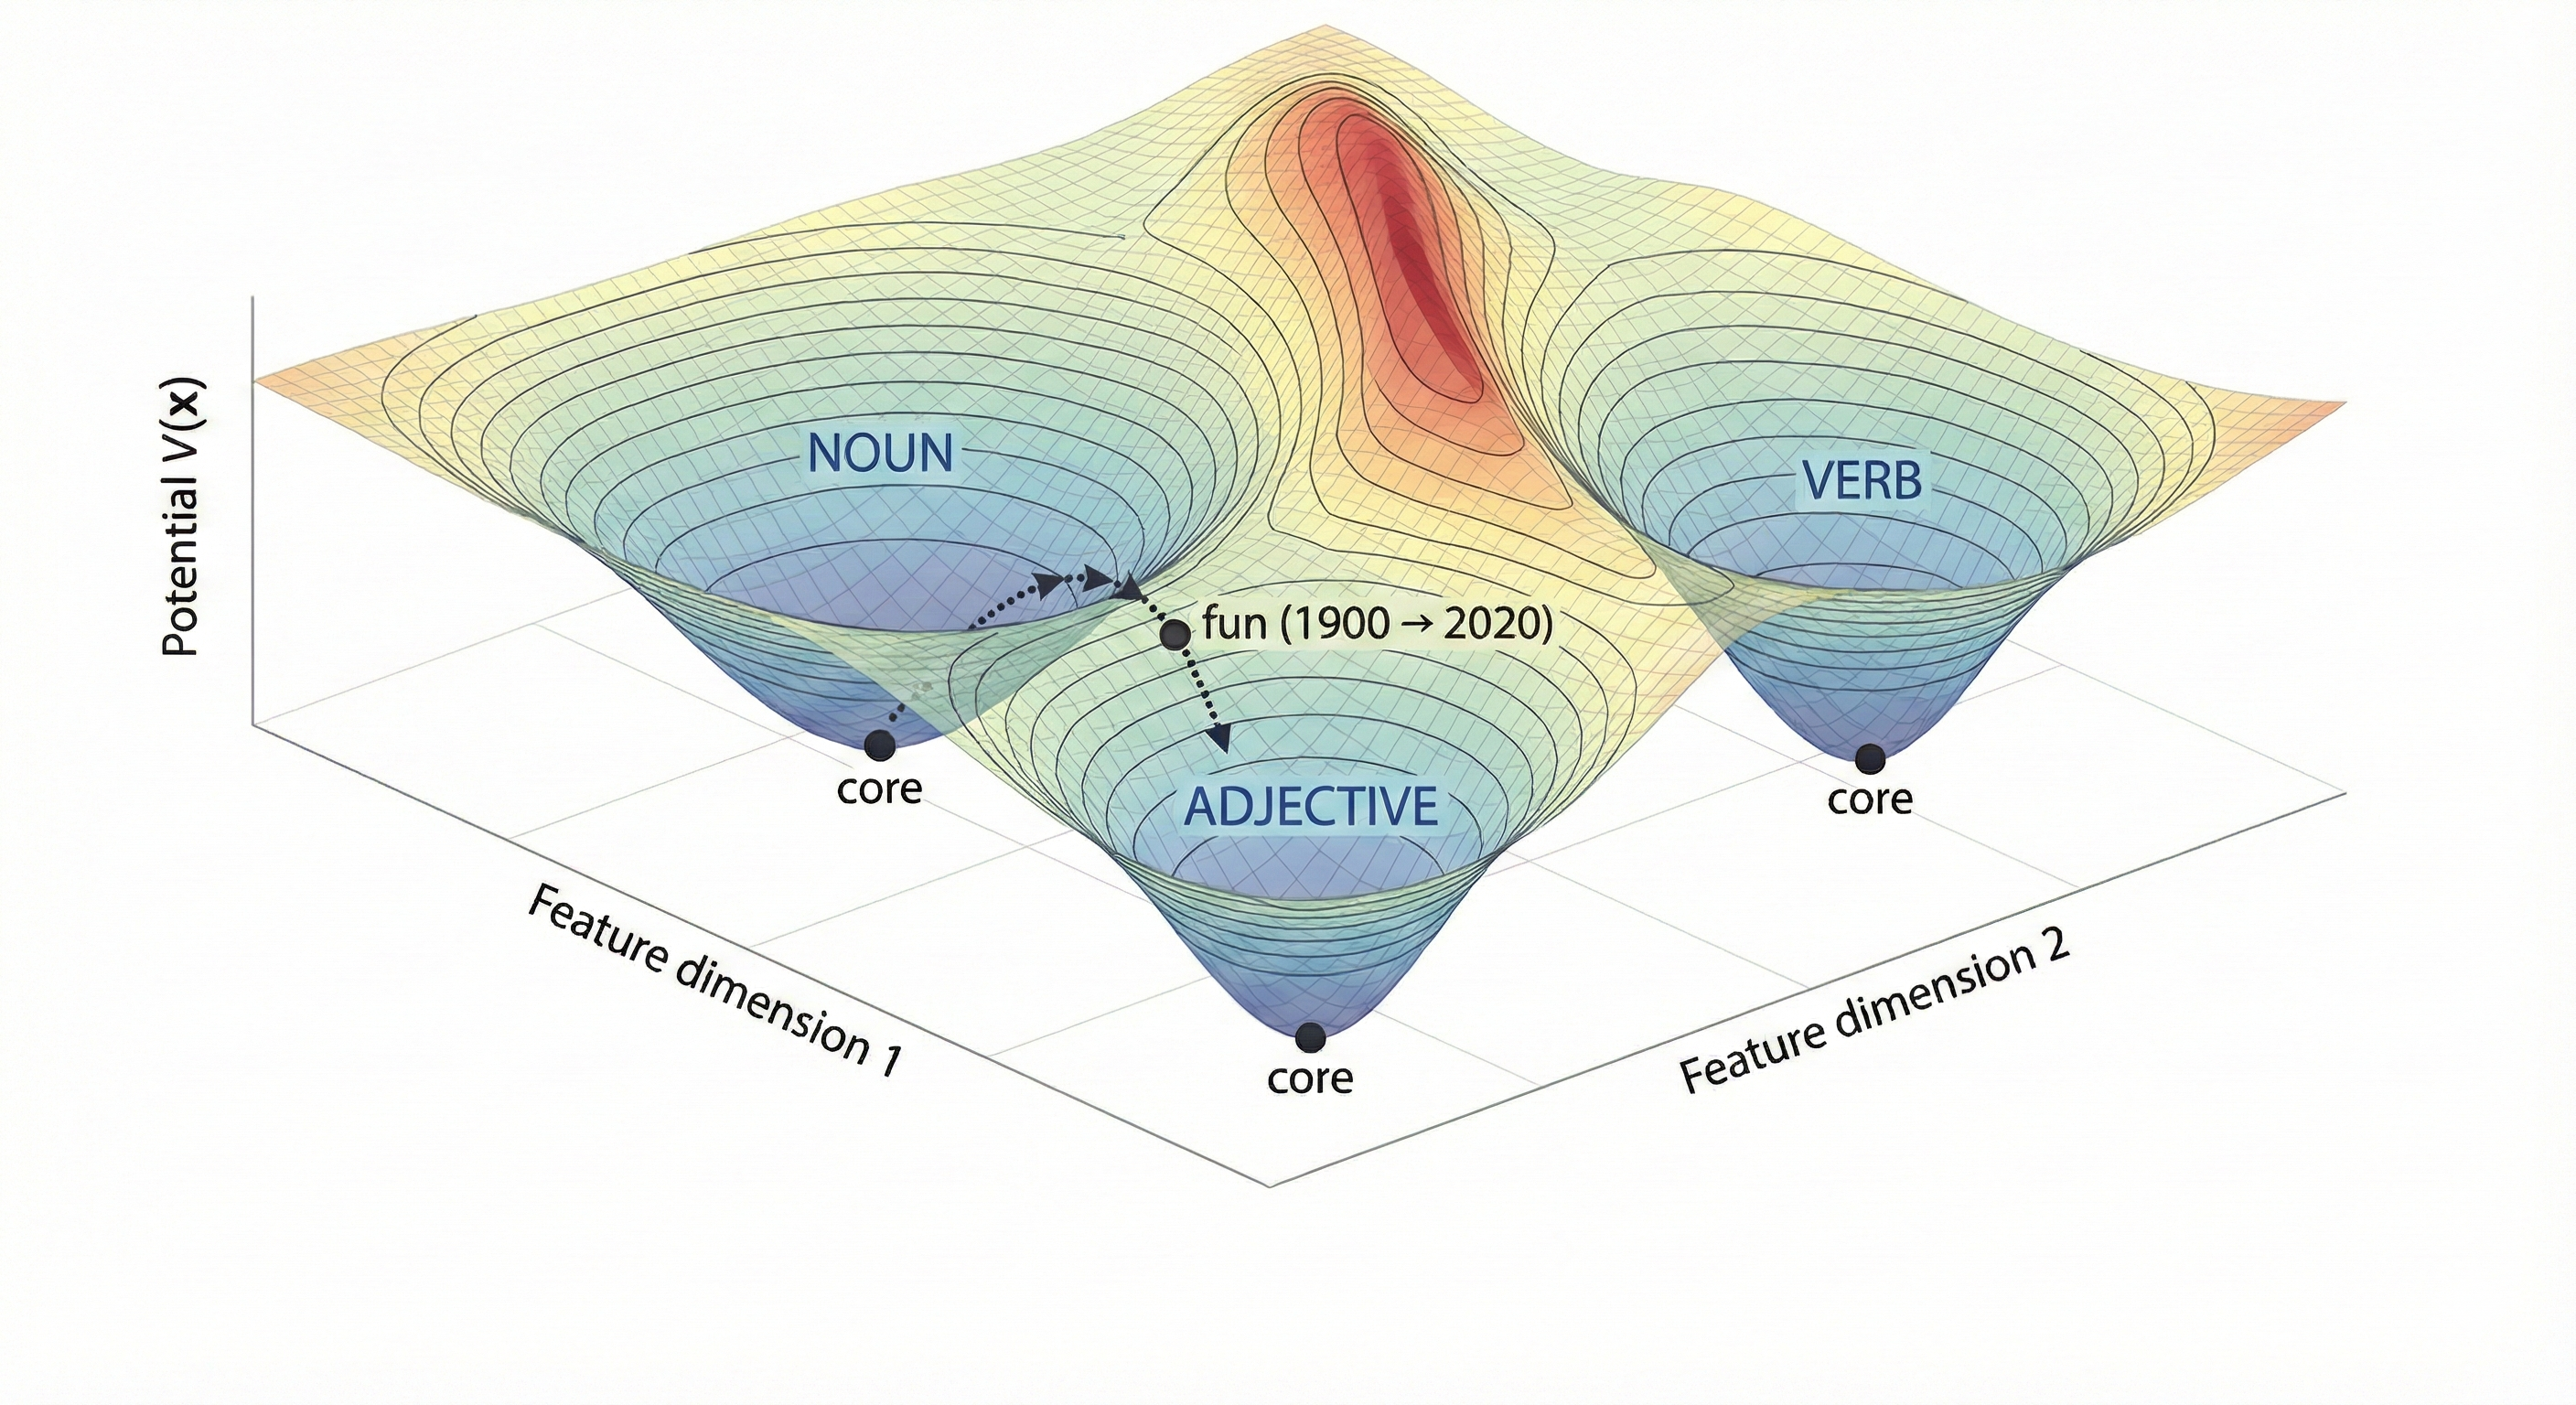
\includegraphics[width=\textwidth]{figures/5.three-basins.png}
\caption{A two-dimensional slice through grammatical feature space, with the potential function $V(\mathbf{x})$ plotted vertically. Category cores correspond to local minima; boundaries to ridges and saddle points. The noun and verb basins are separated by a high ridge (disjoint categories); the noun and adjective basins share a low saddle (porous boundary, overlapping membership possible). The trajectory of \emph{fun} illustrates diachronic movement from deep in the noun basin toward the noun--adjective boundary.}
\label{fig:basin-visualization}
\end{figure}

\paragraph{Basin structure.}
With a metric in hand, the multi-dimensional picture comes into focus. Each category occupies a region in feature space~-- a basin of attraction. Items deep in a basin are stably categorised: small perturbations don't move them out. Items near the boundary are unstable: the same perturbation that would be negligible elsewhere can flip the categorization.

The basins are typically convex. If two items are stably categorised as nouns, items intermediate between them in feature space should generally be too. This is Gärdenfors's criterion for natural categories, and it holds here because the mechanisms maintaining the basin~-- entrenchment, analogy, transmission~-- operate by similarity. Items near the prototype pull their neighbours toward the same categorisation. Apparent non-convexity, where it arises, may indicate that the relevant metric isn't the one assumed, that multiple overlapping basins are being conflated, or that the category has a multi-peaked structure~-- each of these is informative about the mechanisms at work.

The potential-well metaphor captures this: a convex basin corresponds to a single local minimum, and gradient descent from anywhere in the basin leads to the same attractor.

The boundary cases that trouble essentialism~-- \mention{fun}, \mention{near}, \mention{otherwise}~-- are items near basin boundaries. They exhibit properties of multiple categories because they're in the region where tolerance breaks down. Their instability isn't noise; it's evidence about where the boundaries lie.

The maintained categories behave as if they have sharp decision boundaries under ordinary measurement regimes; what is graded is stability and typicality, not membership. At any point in feature space, an item is either in category $i$ or not under the mechanisms currently in play. The appearance of gradience arises partly from epistemic limitations~-- we observe items at various distances from boundaries and cannot determine exactly where the boundaries fall~-- but also from \emph{synchronic context effects}. The same word may be perceived as more noun-ish or adjective-ish depending on the syntactic frame; the same phoneme may shift category depending on rate-normalised expectations. The basin metaphor accommodates this: mechanisms set the default landscape, but context induces local deformations. Think of the terrain not as a static watershed but as something that flexes moment-to-moment, with items pulled toward or away from boundaries by the cues available in the immediate environment. This is \term{real gradience}~-- gradient structure that is genuine evidence about category organisation, not noise to be explained away.

\subsection{Mechanisms and basins}
\label{subsec:5:mechanisms-basins}

The hyperreal model describes the geometry of category boundaries. The HPC framework describes what maintains that geometry. The two are complementary.

Two stories, then. The first is representational: grammatical categories are regions in a feature space, with prototypes at centres and boundaries where similarity to multiple prototypes is balanced. This is the geometry.

The second is causal: the geometry persists because mechanisms~-- acquisition, entrenchment, alignment, transmission, functional pressure~-- exert forces that keep items clustered and boundaries stable. Conceptual-space approaches develop the first story in rich detail \citep{gardenfors2000,gardenfors2014}; HPC frameworks develop the second \citep{boyd1991,boyd1999}.

Both are needed. The geometry tells you what shape the categories have. The mechanisms tell you why they hold that shape.

Rosch's insight that categories have graded internal structure organised around prototypes is preserved~-- but repurposed. What's graded is typicality, not membership. An item is in the category or out; that boundary is sharp. But items inside the category vary in how typical they are, how central to the basin, how far from competing boundaries. HPC retains the gradience while relocating it: not degrees of membership but degrees of stability. A typical noun is one that sits deep in the noun basin, far from competition; an atypical noun sits nearer a boundary, more vulnerable to drift, eruptions, erosion. The mechanisms~-- entrenchment, alignment, transmission~-- are the forces that maintain this structure.

The hyperreal formalisation adds precision about boundaries: sharp but located at unreachable distances, exactly as tolerance intuitions suggest. Prototype theory describes the shape; HPC explains the stability; hyperreals explain the sharpness.

Like the spinning top (Chapter~\ref{ch:kinds-without-essences}), the stability is dynamic, maintained by active forces rather than static rigidity. The homeostatic mechanisms are exactly these stabilising forces. They do not define the boundaries~-- that would be essentialism~-- but they maintain the landscape geometry.

\textbf{Acquisition} shapes the initial configuration: learners sensitive to input distributions reproduce the basin structure. \textbf{Entrenchment} deepens the basins: high-frequency items anchor the category, steepening the walls around the prototype.

\textbf{Interactive alignment} maintains consistency: speakers coordinate usage, effectively pushing deviants back toward the norm. Consider alignment in action. Suppose you say \mention{that was very fun}~-- using the degree modifier that signals adjectival status. Your interlocutor might accommodate, adopting \mention{very fun} in their next turn. Or they might resist, persisting with \mention{a lot of fun}. Either way, the micro-choice shifts local expectations: accommodation reinforces the adjectival pattern; resistance maintains the nominal one. Scale this up, and you get a distributed mechanism for maintaining shared norms.

\textbf{Iterated transmission} acts as a filter across generations. Not all variants survive; the ones that do tend to be clear exemplars well inside basins. As \citet{kirby2008} demonstrated, transmission bottlenecks can select for learnable structures. In their experimental evolution of artificial languages, random mappings became compositional over ten generations because the bottleneck of imperfect learning filtered out the arbitrary variants (Figure~\ref{fig:iterated-learning}). This pattern is not inevitable~-- it depends on particular task pressures and on the right balance of expressivity and compressibility~-- but it illustrates how structure can emerge without intentional design.

Finally, \textbf{functional pressure} ensures the basins serve communicative needs. Categories exist because they package referents or encode events. Where functional pressure is strong, basins are deep and boundaries are sharp.

All these forces act together to maintain the basin geometry. The hyperreal model describes the shape; the mechanisms explain why it holds.

The hyperreal model tells us what the basin structure looks like: sharp thresholds with scale-dependent tolerance, and instability concentrated in a determinate seam-region that ordinary finite measurement cannot pinpoint. The HPC framework tells us why the structure persists: mechanisms operating across multiple timescales, maintaining the clustering without defining it.

\subsection{Multi-category spaces}
\label{subsec:5:multi-category}

Linguistic categories don't exist in isolation. Nouns compete with verbs; adjectives shade into adverbs; prepositions overlap with both. Instead of a set of independent regions, the basin structure is a tessellation of feature space, with categories abutting each other along shared boundaries. Khalidi calls such overlapping classification schemes \term{crosscutting kinds} and argues they pose no threat to realism: the same entity can be a node in multiple causal networks simultaneously \citep[69--72, 92--97]{khalidi2013}.
This creates additional structure. An item near the noun-verb boundary might be stably a noun (because it's deep in the noun basin) or unstably categorized (because small changes could push it into the verb basin). The same item might be far from the noun-adjective boundary, so its nominal vs.\ adjectival status is never in doubt. Category membership is determinate in multiple dimensions simultaneously, with different degrees of stability in different directions.

Consider the data for \mention{fun}~-- for fun, as it were. In the frequency-of-degree-modification dimension, it has drifted toward adjectives: \mention{very fun} is increasingly acceptable. In the takes-a-determiner dimension, it remains nominal: \mention{the fun we had} is unremarkable. The item sits near the noun-adjective boundary in one dimension, deep in noun territory in another. Its apparent mixed status reflects its location in a multi-dimensional space, not indeterminacy about what categories are.

American historical corpus evidence makes the trajectory visible \citep{davies2010coha}. Degree-modified \mention{fun}~-- \mention{really fun}, \mention{so fun}, \mention{rather fun}, \mention{very fun}~-- is rare through most of the 19th and early 20th centuries but rises sharply from the late 20th century onward (Figure~\ref{fig:fun-coha}). The pattern is consistent with a shift from marginal adjectival-like uses to robust productivity. \mention{Rather fun} shows early isolated footholds (British epistolary usage appears as early as 1827); the American surge comes later. The diagnostics co-move: this is not one fragile string but a bundle of degree environments converging in the same direction.

\begin{figure}[t]
\centering
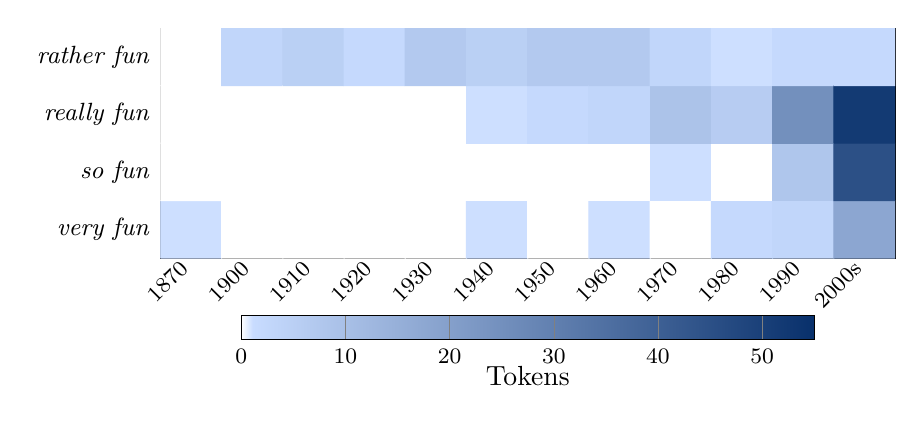
\begin{tikzpicture}
\begin{axis}[
    width=0.9\textwidth,
    height=4.5cm,
    view={0}{90},
    colorbar horizontal,
    colorbar style={
        at={(0.5,-0.25)},
        anchor=north,
        width=0.6\textwidth,
        height=0.3cm,
        xlabel={Tokens},
        xlabel style={yshift=0.2cm},
        xticklabel style={font=\footnotesize},
    },
    colormap={WhiteBlue}{rgb255(0cm)=(255,255,255); rgb255(0.02cm)=(200,220,255); rgb255(1cm)=(8,48,107)},
    colormap name=WhiteBlue,
    point meta min=0,
    point meta max=55,
    xtick={1,2,3,4,5,6,7,8,9,10,11,12},
    xticklabels={1870,1900,1910,1920,1930,1940,1950,1960,1970,1980,1990,2000s},
    xticklabel style={font=\footnotesize, rotate=45, anchor=east},
    ytick={1,2,3,4},
    yticklabels={\textit{very fun},\textit{so fun},\textit{really fun},\textit{rather fun}},
    yticklabel style={font=\small},
    xlabel={},
    ylabel={},
    enlargelimits=false,
]
% Data matrix: rows = modifiers (bottom to top: very, so, really, rather)
% columns = decades (1870, 1900, 1910, 1920, 1930, 1940, 1950, 1960, 1970, 1980, 1990, 2000s)
% 2000s combines 2000 and 2010 since those are the surge years
\addplot[matrix plot*, mesh/cols=12, point meta=explicit] coordinates {
    % very fun: 1870=1, gaps, 1940=1, 1960=1, 1980=2, 1990=3, 2000s=18
    (1,1) [1]  (2,1) [0]  (3,1) [0]  (4,1) [0]  (5,1) [0]  (6,1) [1]  (7,1) [0]  (8,1) [1]  (9,1) [0]  (10,1) [2]  (11,1) [3]  (12,1) [18]
    % so fun: late surge
    (1,2) [0]  (2,2) [0]  (3,2) [0]  (4,2) [0]  (5,2) [0]  (6,2) [0]  (7,2) [0]  (8,2) [0]  (9,2) [1]  (10,2) [0]  (11,2) [8]  (12,2) [45]
    % really fun: late surge
    (1,3) [0]  (2,3) [0]  (3,3) [0]  (4,3) [0]  (5,3) [0]  (6,3) [1]  (7,3) [2]  (8,3) [3]  (9,3) [9]  (10,3) [6]  (11,3) [25]  (12,3) [52]
    % rather fun: steady early, declines (now row 4 = top)
    (1,4) [0]  (2,4) [3]  (3,4) [5]  (4,4) [2]  (5,4) [7]  (6,4) [5]  (7,4) [7]  (8,4) [7]  (9,4) [3]  (10,4) [1]  (11,4) [2]  (12,4) [2]
};
\end{axis}
\end{tikzpicture}
\caption{Degree-modified \mention{fun} in the Corpus of Historical American English. Darker cells indicate higher frequency. \mention{Rather fun} shows scattered early attestations; \mention{really fun} and \mention{so fun} surge in the 1990s--2000s. The late-century darkening across multiple rows shows convergent adjectivalisation.}
\label{fig:fun-coha}
\end{figure}

\paragraph{Boundary phenomena: operationalising distance.}
The \mention{fun} example shows diachronic drift toward a boundary. But how do we study items that sit \emph{at} a boundary synchronically~-- stably intermediate, not in transition but genuinely in between?

English reciprocals~-- \mention{each other}, \mention{one another}~-- offer a detailed case study \citep{reynolds2025reciprocals}. Standard reference grammars classify them as pronouns, and their distribution supports that much: they head NP-like phrases in the same slots as core pronouns, as verb and preposition complements. But they are non-canonical pronouns. Unlike core personal pronouns, they lack a person/gender/case paradigm and are distributionally defective in the most salient way: they resist ordinary free subject use (cf. \mention{Somebody left} vs. \mention{*Each other left}). 

On the other side, reciprocals are built from determinative material (\mention{each}/\mention{one}) and impose a determinative-like semantic constraint: they are obligatorily anaphoric and require plural antecedents. Yet they are not determiners: they cannot occur in determiner function (*\mention{each other friends} in the intended sense). My aim is not to force a verdict from a handful of tests, but to motivate the boundary question: reciprocals sit where the pronoun and determinative profiles exert opposed pulls, making them an ideal probe for how to operationalise stable in-betweenness.

How stable is this in-betweenness? The methodology in \citet{reynolds2025reciprocals} addresses exactly this question by applying three diagnostics:

\begin{enumerate}
\item \textbf{Invariance under analytic perturbation.} Does the boundary position shift when you change the distance metric, the comparison set, or the feature weights? Across multiple correspondence analysis ordinations, Jaccard distances, and specification curves, reciprocals sit midway between pronoun and determinative anchors~-- a stable intermediate, not an artefact of a particular operationalisation.

\item \textbf{Cross-dimensional tension.} Do different feature families pull in different directions? Morphology pulls reciprocals toward determinatives (they lack the case paradigm of core pronouns). Semantics pulls them toward pronouns (they denote referents, not quantities). Syntax and phonology contribute little. The signature of a boundary item is exactly this: opposed pulls from mechanisms that maintain different basins.
\item \textbf{Clear anchors behave cleanly.} Do items unambiguously inside each basin show the expected clustering? Core pronouns like \mention{he} and \mention{herself} sit deep in the pronoun basin; determinatives like \mention{every} and \mention{either} sit deep in the determinative basin. The methodology confirms what intuition expects: the anchors cluster where they should. The interesting finding is that reciprocals don't.
\end{enumerate}

A caveat about statistical significance. Whether the boundary position looks \enquote{statistically significant} depends on which comparison items you choose. Pick one reasonable set and the result is extreme; vary the comparison set and the result wobbles. But the \emph{qualitative} finding~-- reciprocals sit between pronoun and determinative anchors~-- is stable across all choices. Under an HPC reading, this is exactly what genuine boundaries should look like: the diagnosis persists, but decisive p-values elude us because the item really is intermediate.

This operationalises the chapter's theoretical picture. \enquote{Distance to boundary} is not metaphorical; it can be measured. \enquote{Stability of ambiguity} is not vague intuition; it is invariance under analytic perturbation~-- the in-betweenness persists when you change your measurement instrument. Reciprocals sit in the overlap region of Figure~\ref{fig:disjoint-overlap}, not because the analysis went wrong but because the basin structure itself has overlap.

The same analysis applies to the existential debates about feature systems raised in §\ref{sec:3:lexeme-obsession}. Is \textsc{gender} a natural kind, or is it reducible to \textsc{number}? The question becomes: do gender and number occupy distinct basins maintained by distinct mechanisms, or is gender a sub-region of a larger number basin, maintained by the same mechanisms at a finer grain?

If the mechanisms maintaining gender systems~-- agreement patterns, acquisition pathways, functional pressures toward nominal classification~-- are distinct from those maintaining number systems, then gender is a genuine natural kind: a separate basin in the space of grammatical features. If the mechanisms overlap substantially~-- if gender turns out to be number's machinery for individuation, as some theorists have argued~-- then the basins merge, and \textsc{gender} as a cross-linguistic category dissolves into \textsc{number}.

This is an empirical question, not a definitional one. The hyperreal model tells us what to look for: distinct basins with sharp thresholds and scale-dependent tolerance. The HPC framework tells us how to investigate: identify the mechanisms, trace their operation, determine whether they cluster distinct properties or the same properties at different scales.

Consider the Shilluk number system introduced in §\ref{sec:3:lexeme-obsession}. English marks number with a suffix: \mention{cat}, \mention{cats}. Shilluk marks it through stem-internal changes in tone, vowel length, and voice quality~-- a singular/plural pair might differ only in whether the vowel is short, long, or overlong, or in whether the tone is Low or Fall. The exponence is lexicalised: each pair must be learned; no productive rule derives one from the other.

What does the HPC + hyperreal view say about this? Both English and Shilluk number systems occupy basins in a feature space whose dimensions include obligatoriness (number must be specified), agreement scope (specifier, verb, other constituents), and semantic function (individuation of entities). The exponence dimension~-- where English is affixal and Shilluk is fusional/suprasegmental~-- places them in different regions of morphophonological space but the same region of morphosyntactic and semantic space. They're in overlapping basins, not identical ones~-- independent systems shaped by similar pressures, not one system shared across languages.

The mechanisms maintaining the two systems are partially shared (acquisition of obligatory contrast, iterated transmission of the singular/non-singular distinction) and partially distinct (rule-based productivity in English, lexical storage in Shilluk). The prediction is that where the mechanisms align~-- the functional pressure to distinguish singular from plural~-- the categories should pattern similarly across languages. Where they diverge~-- the phonological substance of the exponence~-- we should expect variation. That's exactly what we find. The basin boundary for \textsc{number} is sharp in both languages (a noun is singular or plural, not in between), but the basin's location in the full feature space differs, because different mechanisms weight different dimensions. The same analysis extends to noun-class systems like Swahili's, to Mandarin classifiers, to German gender. Wherever there's grammatical categorisation, there should be basin structure maintained by mechanisms.

A question arises: is the cross-linguistic similarity \emph{convergence} or \emph{homology}? In biology, convergence means similar phenotypes arising independently (the wings of bats and birds), while homology means similarity inherited from a common ancestor (the forelimbs of all mammals). For \textsc{number}, the answer is probably convergence: the functional pressure to distinguish singular from plural exists in any language with nominal reference, and different languages have evolved different morphological solutions. The mechanisms overlap not because of common ancestry but because of common function. For \textsc{noun} and \textsc{verb}, the answer might be different: if these categories reflect universal constraints on predication and reference, they may be homologous~-- inherited from whatever cognitive architecture makes human language possible. The framework should distinguish these cases, and the mechanistic analysis provides the tools: shared mechanisms suggest homology; parallel mechanisms suggest convergence.

If the HPC analysis just confirms that English number and Shilluk number are both \textsc{number}, have we learned anything? Yes: the framework explains \emph{why} they deserve the same label~-- not definitional fiat, but overlapping mechanisms maintaining overlapping basins. And it makes predictions: if we found a putative \enquote{number} category maintained by entirely different mechanisms with no overlap in the functional dimension, the framework would say it's not the same kind~-- same label, different basin.

\section{Empirical consequences}
\label{sec:5:empirical-consequences}

\subsection{Gradient judgments, discrete categories}
\label{subsec:5:gradient-discrete}

The discreteness problem has a close cousin: the gradient-judgment problem. Speakers' acceptability judgments are notoriously gradient. Asked to rate sentences on a 1--7 scale, they distribute across the range, with clear acceptability at the extremes and uncertainty in the middle. If categories are discrete, why are judgments gradient?

The hyperreal framework suggests an answer. Distinguish the category from its measurement, the ontology from its epistemology.

\textbf{Grammaticality}~-- the property of conforming to the grammar~-- is discrete. A sentence either satisfies the constraints or it doesn't. The boundary between grammatical and ungrammatical is sharp, located at a hyperreal threshold in some underlying dimension (perhaps accumulated constraint violation, or distance from prototype, or processing cost).

\textbf{Acceptability}~-- the measured response in judgment tasks~-- reflects grammaticality filtered through noise. Processing difficulty, frequency effects, task demands, individual variation, and measurement error all intervene between the discrete category and the gradient response. This is where the maintenance framework bites: grammaticality is the maintained category, acceptability is a noisy instrument whose bias terms are themselves mechanism-sensitive (frequency shapes entrenchment, task framing activates different basin configurations, exposure history shapes where the boundary lies for each speaker).

One reason this distinction is so easy to lose sight of is that the phenomenology is asymmetric. When a sentence is well-formed, nothing in particular announces itself: processing just runs. The felt data are mostly negative~-- the \enquote{catch} of a violation, the extra effort, the moment of repair. There is, in that sense, no positive feeling of grammaticality, just as there is no feeling of having sufficient oxygen; the experiences that demand attention are the absences. This is why boundary detection is cognitively natural: violations have a signature, conformity is typically silent.

A second reason is methodological. Temperature is not something you see; it is a theoretical magnitude inferred from what thermometers do. Likewise grammaticality is a latent property that we access only through instruments~-- judgments, reaction times, eye movements, priming, production choices~-- each of which can misread the target in both directions, yielding false comfort (illusory well-formedness) or false alarm (grammatical but degraded). The point is clearest in \emph{satiation} effects: repeated exposure can raise acceptability for initially degraded strings, even though it is implausible that the grammar itself has been rewritten over the course of a short experimental session. Satiation is therefore not a nuisance; it is direct evidence that the mapping from grammaticality to felt acceptability is plastic, and that we should not identify the construct with any one measurement channel.

Not all of these factors work the same way. Random fluctuations~-- trial-to-trial variation in attention, incidental processing load, measurement noise~-- blur the signal without shifting it. But frequency effects and task demands can systematically shift the mapping from grammaticality to acceptability. A borderline construction may be judged more acceptable if it's high-frequency than if it's low-frequency, even when both are equally grammatical. Instructions emphasising naturalness may locate the boundary differently than instructions emphasising correctness. These are biases, not noise. The two-layer model accommodates them: different contexts may activate different effective basin configurations, shifting where tolerance breaks down.

This predicts:
\begin{itemize}
\item Clear cases cluster at scale extremes (1s and 7s), because items deep in the grammatical or ungrammatical basin are stably categorized and noise doesn't flip them.
\item Borderline cases distribute across the middle, because items near the boundary are sensitive to noise~-- small processing fluctuations can shift judgments in either direction.
\item The gradient spread is widest near the boundary, because that's where the signal-to-noise ratio is lowest (see Figures~\ref{fig:two-layer-model} and~\ref{fig:judgment-variance}).
\end{itemize}

This is a testable prediction. If the two-layer model is right, items independently rated as near category boundaries should show higher variance in acceptability judgments than items rated as central. The prediction isn't that boundary items get middling ratings~-- that's compatible with gradient grammaticality~-- but that their ratings should be more variable across trials and subjects. In the simplest latent-threshold models, variance is maximised in the boundary region and falls off as items move deeper into either basin. The exact functional form depends on the measurement channel (binary choice vs.\ rating scale), the noise model, and the way context deforms the local landscape; what is robust is the qualitative signature: variance tracks proximity to the seam. Existing work on gradient acceptability already points in this direction: \citet{sprouse2013} found that judgment variability correlates with distance from prototypical (un)grammaticality, and \citet{dabrowska2010} showed systematic individual differences in judgments of complex constructions~-- exactly what you'd expect if different speakers have slightly different basin structures.

This last point deserves emphasis. The basin structure isn't uniform across speakers. Speakers with different input histories~-- more or less exposure to written registers, different dialectal backgrounds, varying levels of literacy~-- will have basins with different shapes and different boundary locations. The hyperreal model accommodates this naturally: each speaker's grammar is a different model, with a different boundary index $K$. What varies across speakers isn't just noise; it's the underlying geometry. The framework predicts that variability in judgments should be highest for constructions that fall near the boundary \emph{for most speakers}~-- and that speakers who agree on central cases may nonetheless diverge on peripheral ones, because their boundaries are located at different hyperreal indices.

\begin{figure}[t]
\centering
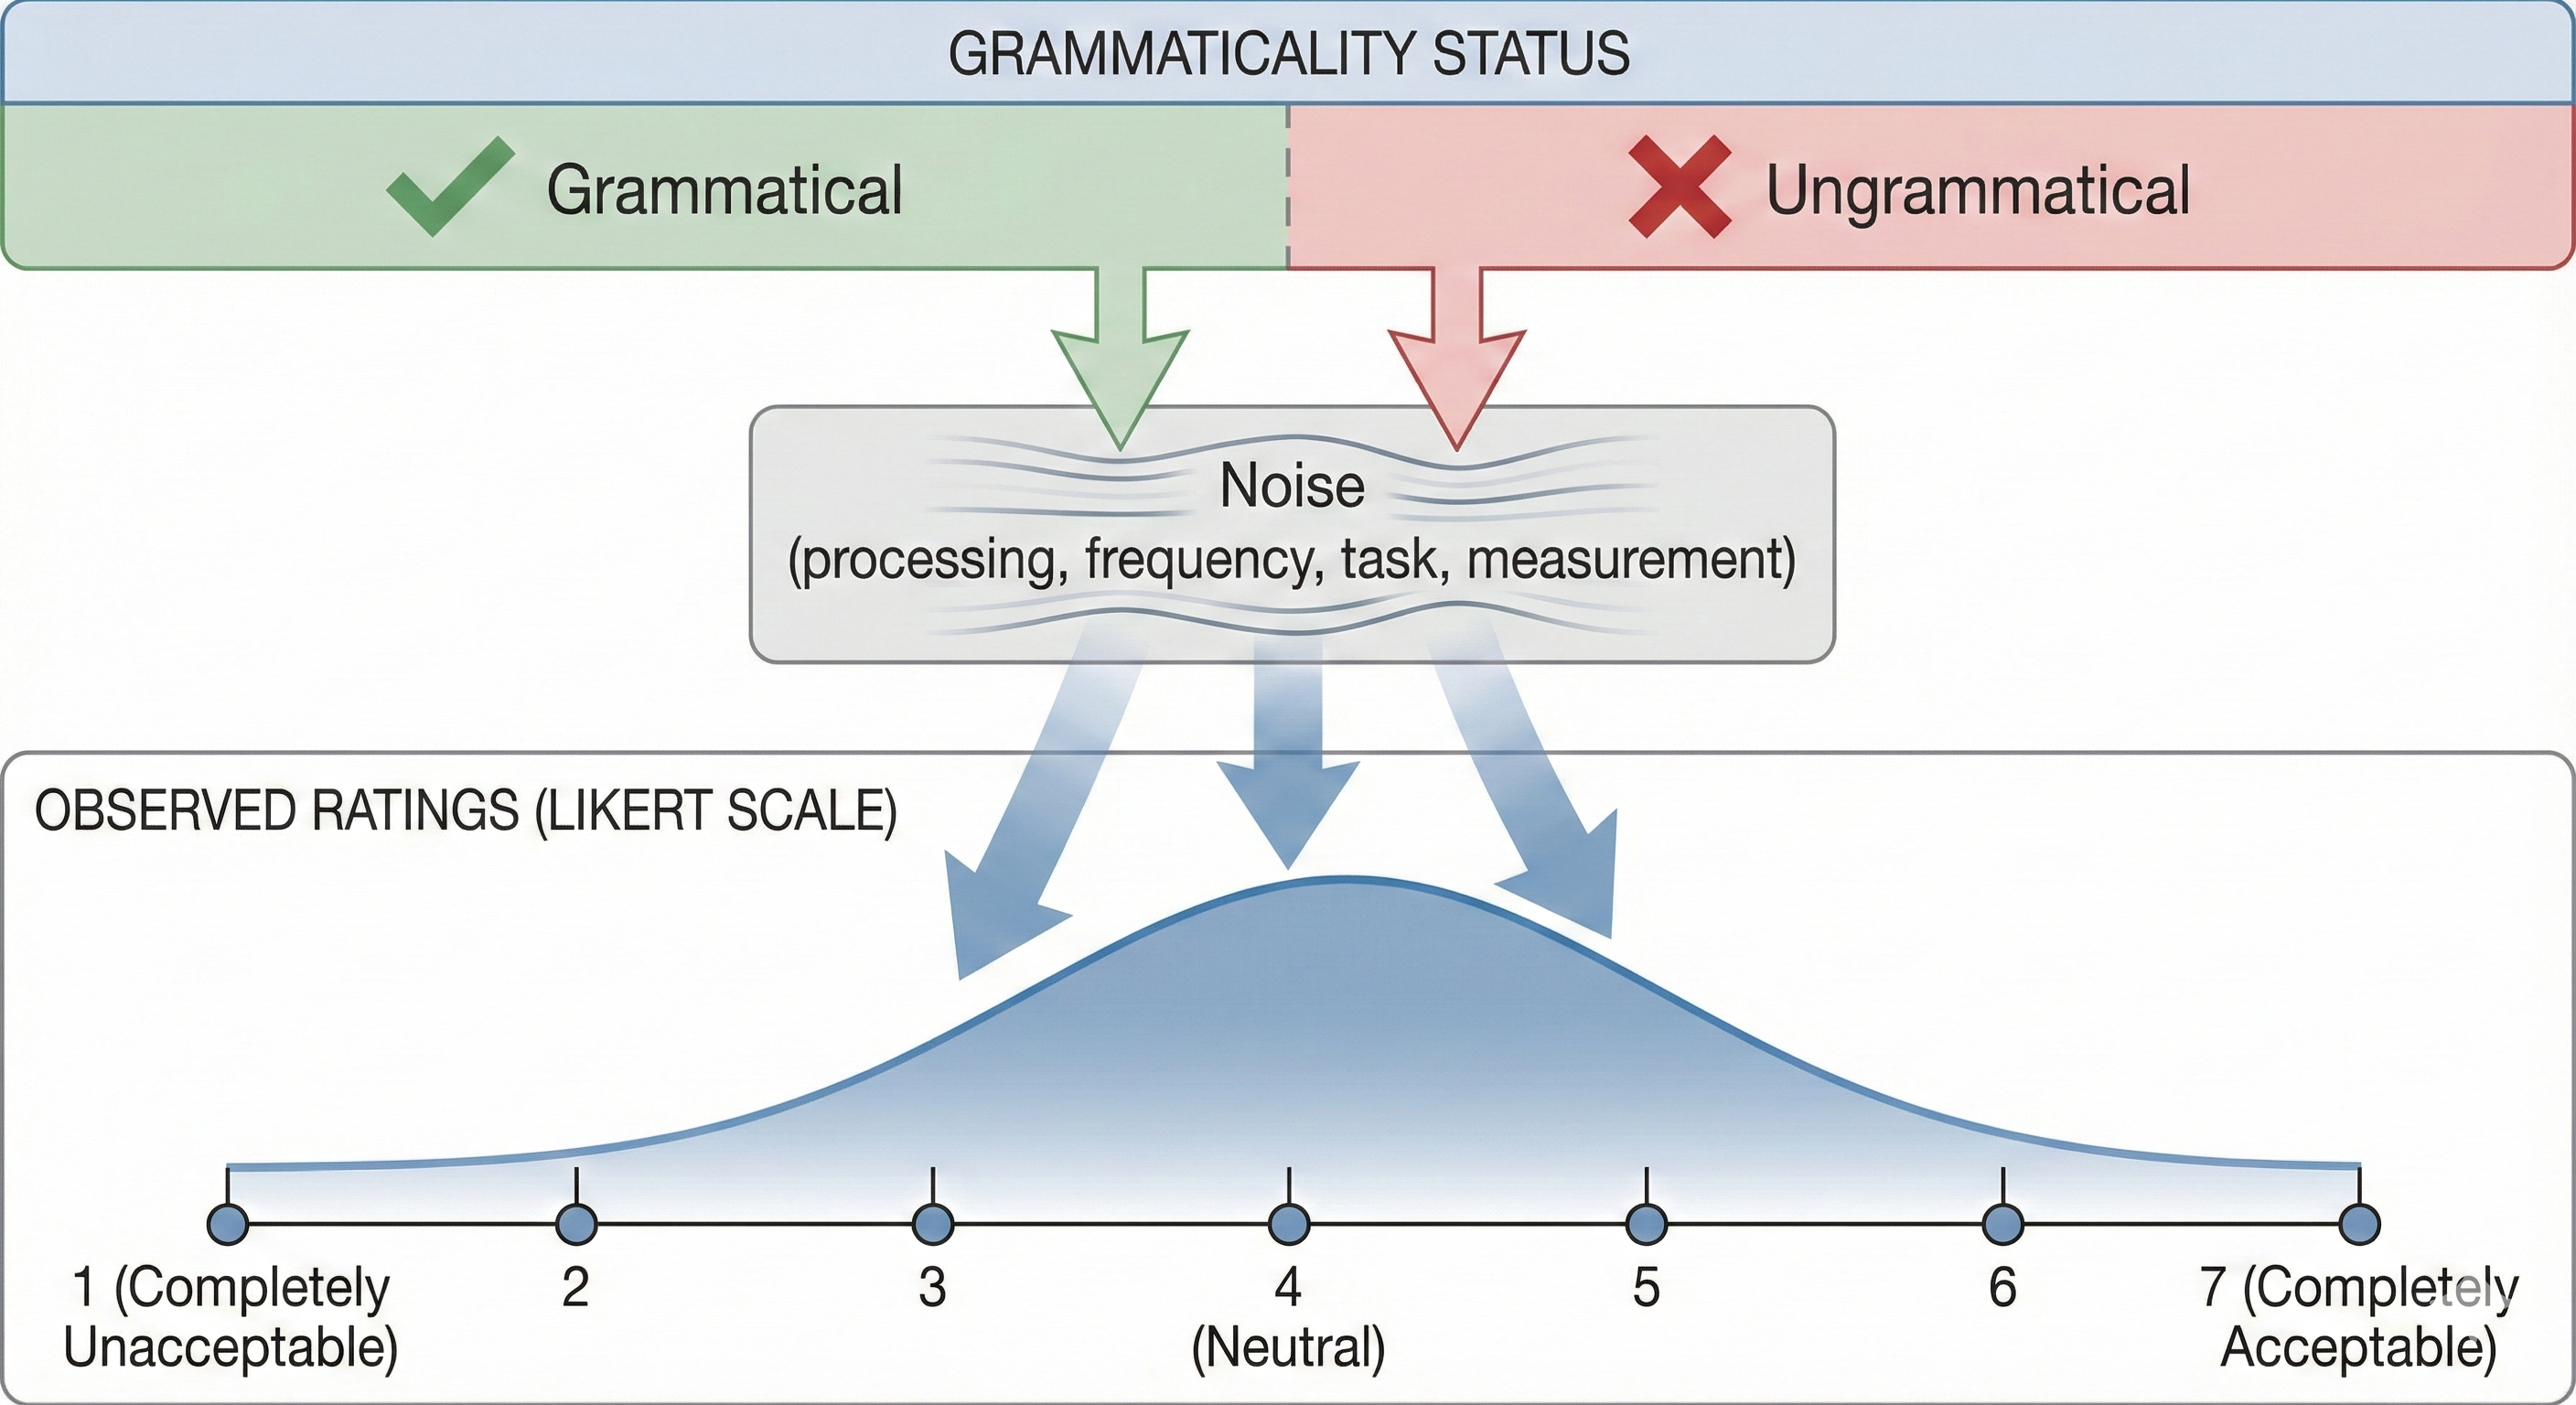
\includegraphics[width=0.85\textwidth]{figures/5.two-layer-grammaticality.png}
\caption{The two-layer model. Discrete grammaticality (binary: grammatical or ungrammatical) is filtered through processing and measurement noise to produce gradient acceptability judgments. Items deep in basins produce stable judgments at scale extremes; items near boundaries produce variable judgments distributed across the middle of the scale.}
\label{fig:two-layer-model}
\end{figure}

\begin{figure}[t]
\centering
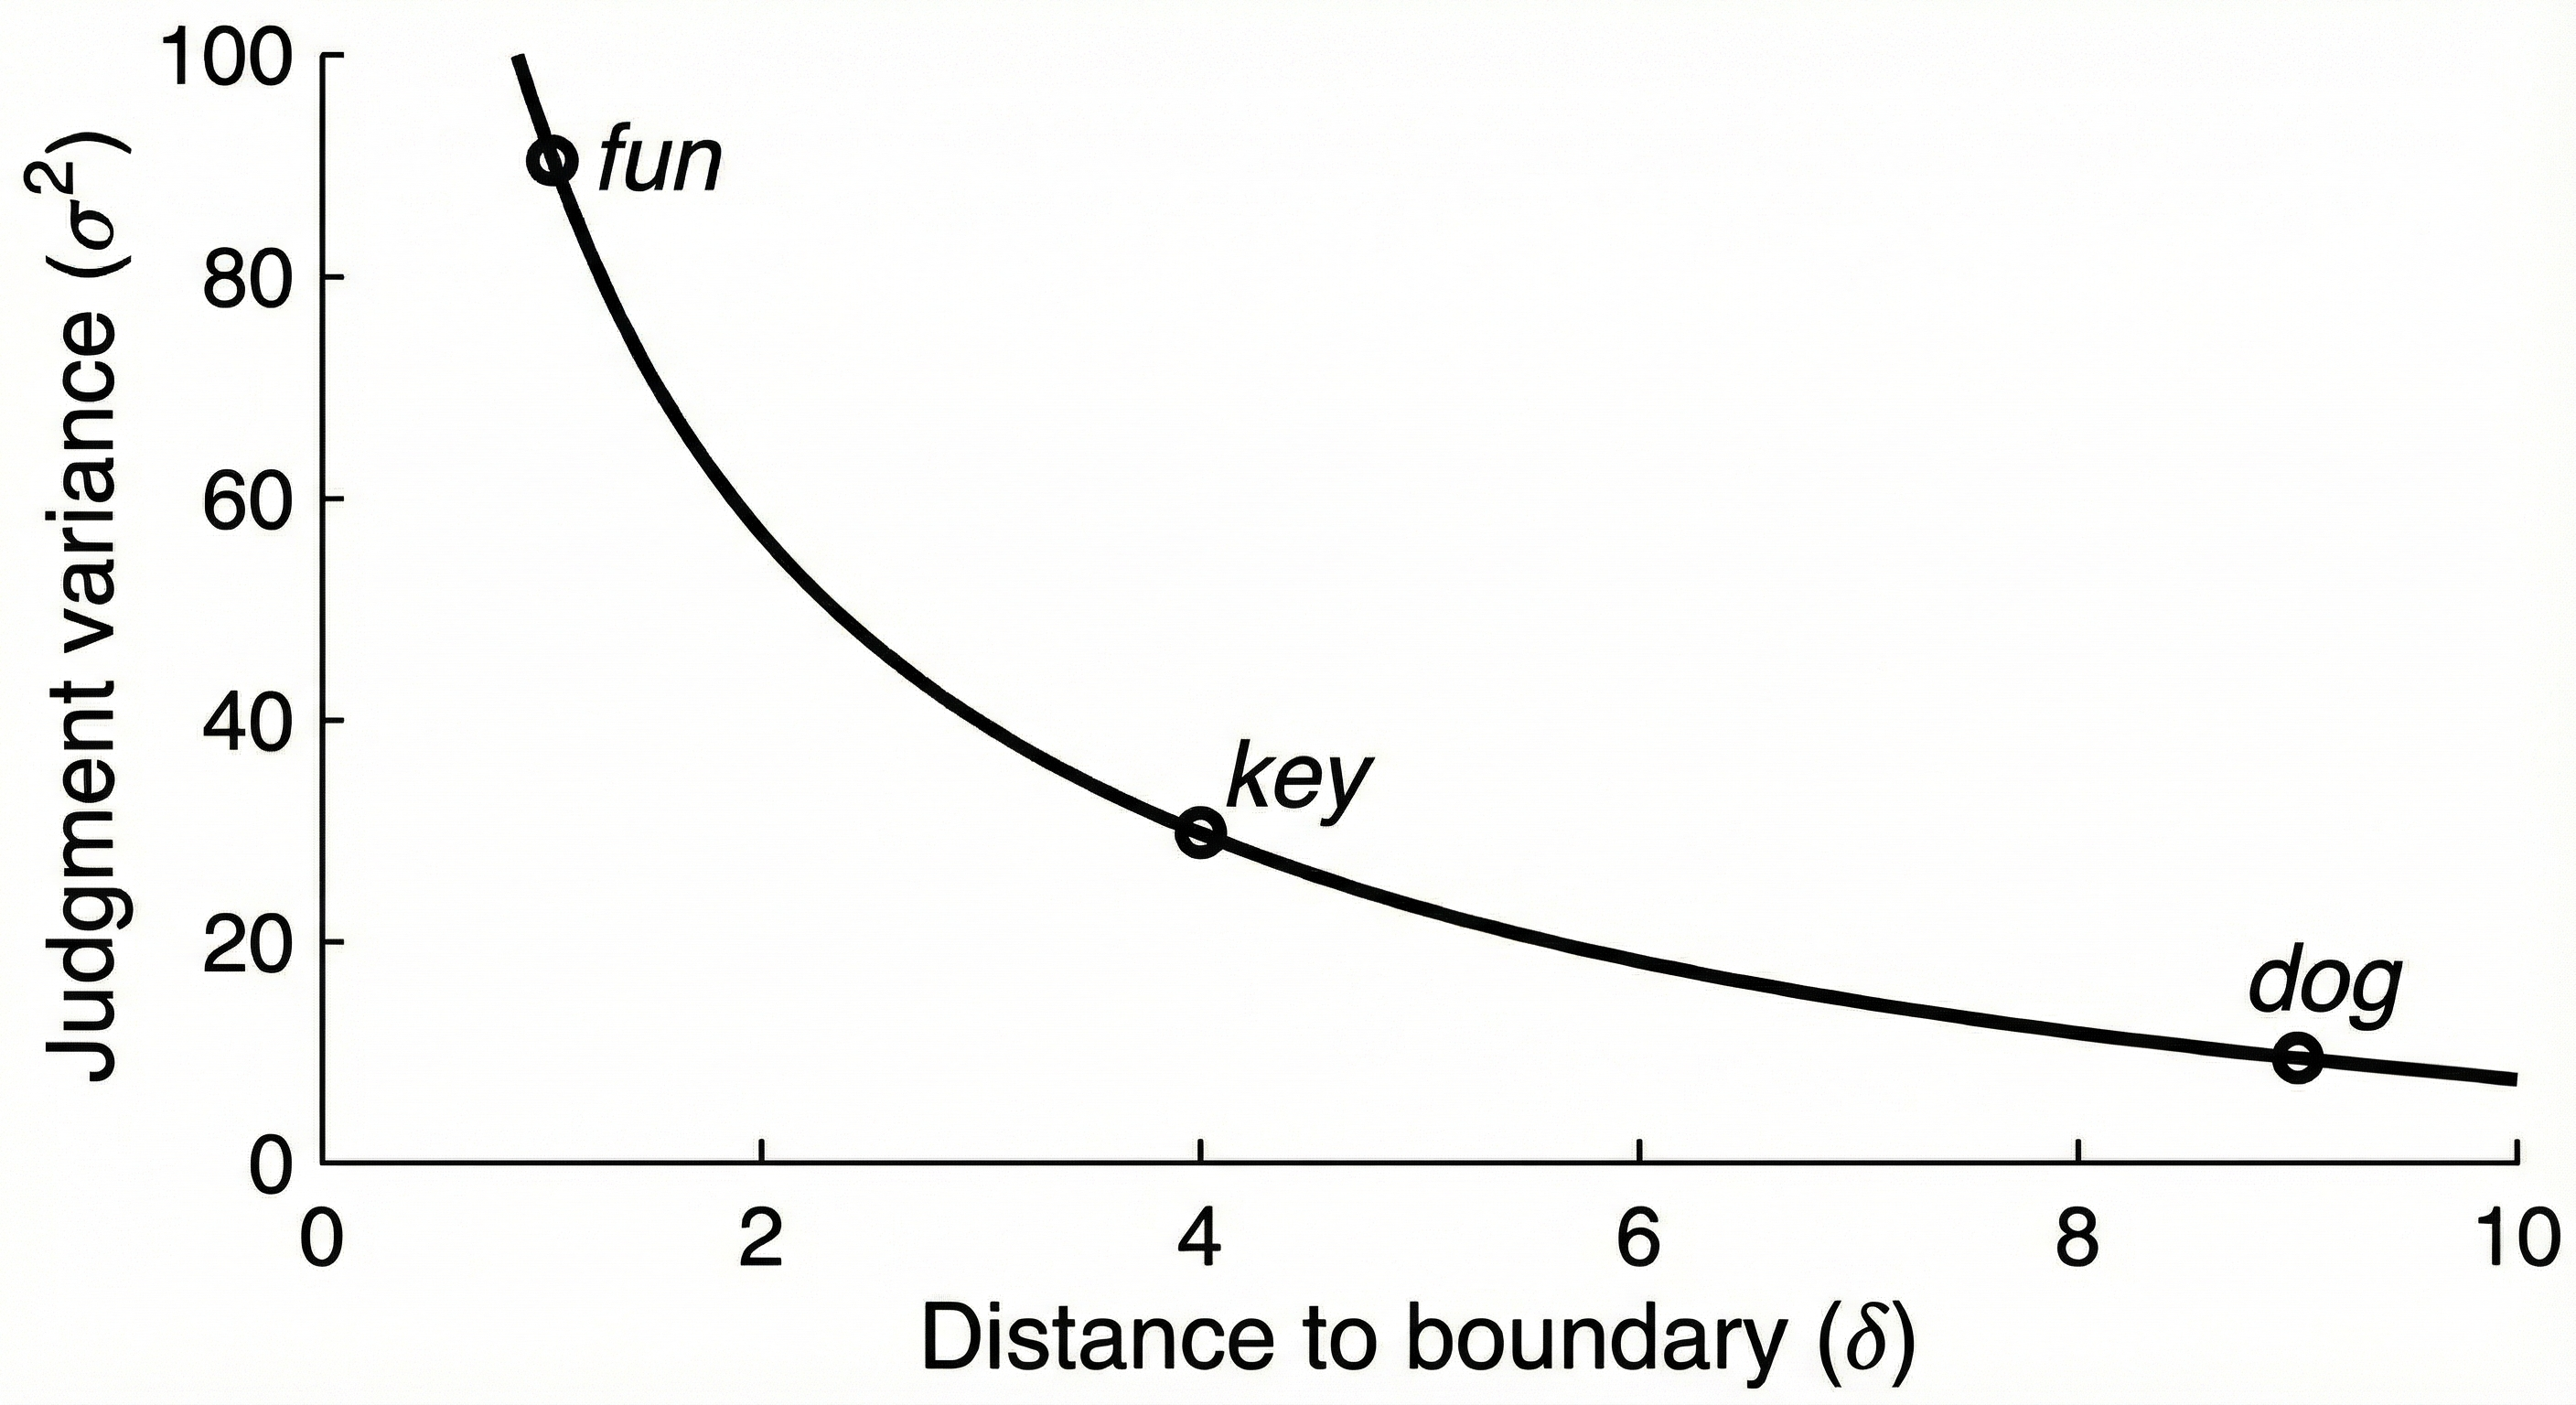
\includegraphics[width=0.85\textwidth]{figures/5.judgment-variance.png}
\caption{Predicted relationship between distance to category boundary and acceptability judgment variance. Items deep in basins (e.g., \mention{dog}) show stable judgments with low variance; items near boundaries (e.g., \mention{near}) show high variability. The qualitative signature~-- variance peaking near the boundary and falling off into each basin~-- is robust; the exact functional form depends on the measurement channel and noise model.}
\label{fig:judgment-variance}
\end{figure}

This is not a new observation~-- the distinction between competence and performance has been with us since Chomsky. But the hyperreal framework adds precision. The boundary is not merely \enquote{somewhere in the grammar}; it's located at a specific (if unspecifiable) hyperreal threshold. The gradience is not merely \enquote{performance noise}; it's the predictable consequence of epistemic limitations near a sharp boundary.

Chapter~\ref{ch:grammaticality-itself} develops this picture fully, arguing that grammaticality itself is a homeostatic property cluster~-- a category maintained by mechanisms, with a sharp boundary at hyperreal distance. For now, the point is that gradient judgments and discrete categories are compatible. The discreteness is in the structure; the gradience is in our access to it.

\subsection{Dual membership}
\label{subsec:5:dual-membership}

One puzzle remains. If categories are discrete~-- if at every point in feature space an item is either in or out~-- how can there be genuine dual membership? How can \mention{near} be both a preposition and an adjective, not contextually selected, not in transition, but stably both? English is comfortable with a kind of dual citizenship here: items like \mention{near} can hold both passports without being in transit.

The answer is that discreteness holds predicate-by-predicate, not across predicates. The predicates \textit{is a preposition} and \textit{is an adjective} are each bivalent: at any point, each is either true or false. But they're not mutually exclusive. The basins can overlap.

This follows naturally from the HPC framework. Categories are maintained by mechanisms, not defined by partition. The mechanisms maintaining prepositionhood~-- patterns of complementation, head-of-PP status, lack of degree modification~-- are partially independent of those maintaining adjectivehood~-- gradability, predicative use, comparative morphology. An item can fall within the tolerance threshold for both, satisfying the clustering criteria for each.

Where the mechanisms align, the basins are disjoint: nouns and verbs occupy separate regions because the mechanisms that maintain them pull in different directions (Figure~\ref{fig:disjoint-overlap}, left). Where the mechanisms cross, the basins overlap: adjectives and prepositions share enough properties~-- predicative function, modification of nominals~-- that some items cluster with both (Figure~\ref{fig:disjoint-overlap}, right).

The regions of overlap are not arbitrary. They're located where the property clusters themselves overlap~-- where an item can satisfy the tolerance criteria for both categories simultaneously. These are exactly the cases that trouble essentialism: items that have \enquote{mixed} status because they satisfy criteria for multiple categories. On the HPC + hyperreal view, mixed status is not indeterminacy but dual location: the item is in two basins at once, stably, because the mechanisms that maintain each basin both apply.

The reciprocals case from §\ref{subsec:5:multi-category} exemplifies this cleanly. Morphology maintains the determinative basin; semantics maintains the pronoun basin. Reciprocals satisfy both. The mixture weights from the blend model~-- 0.534 pronoun-like for \mention{each other}, 0.487 for \mention{one another}~-- are not noise or measurement error. They are the empirical signature of genuine dual location: stable membership in overlapping basins, maintained by partially independent mechanisms.

\begin{figure}[t]
\centering
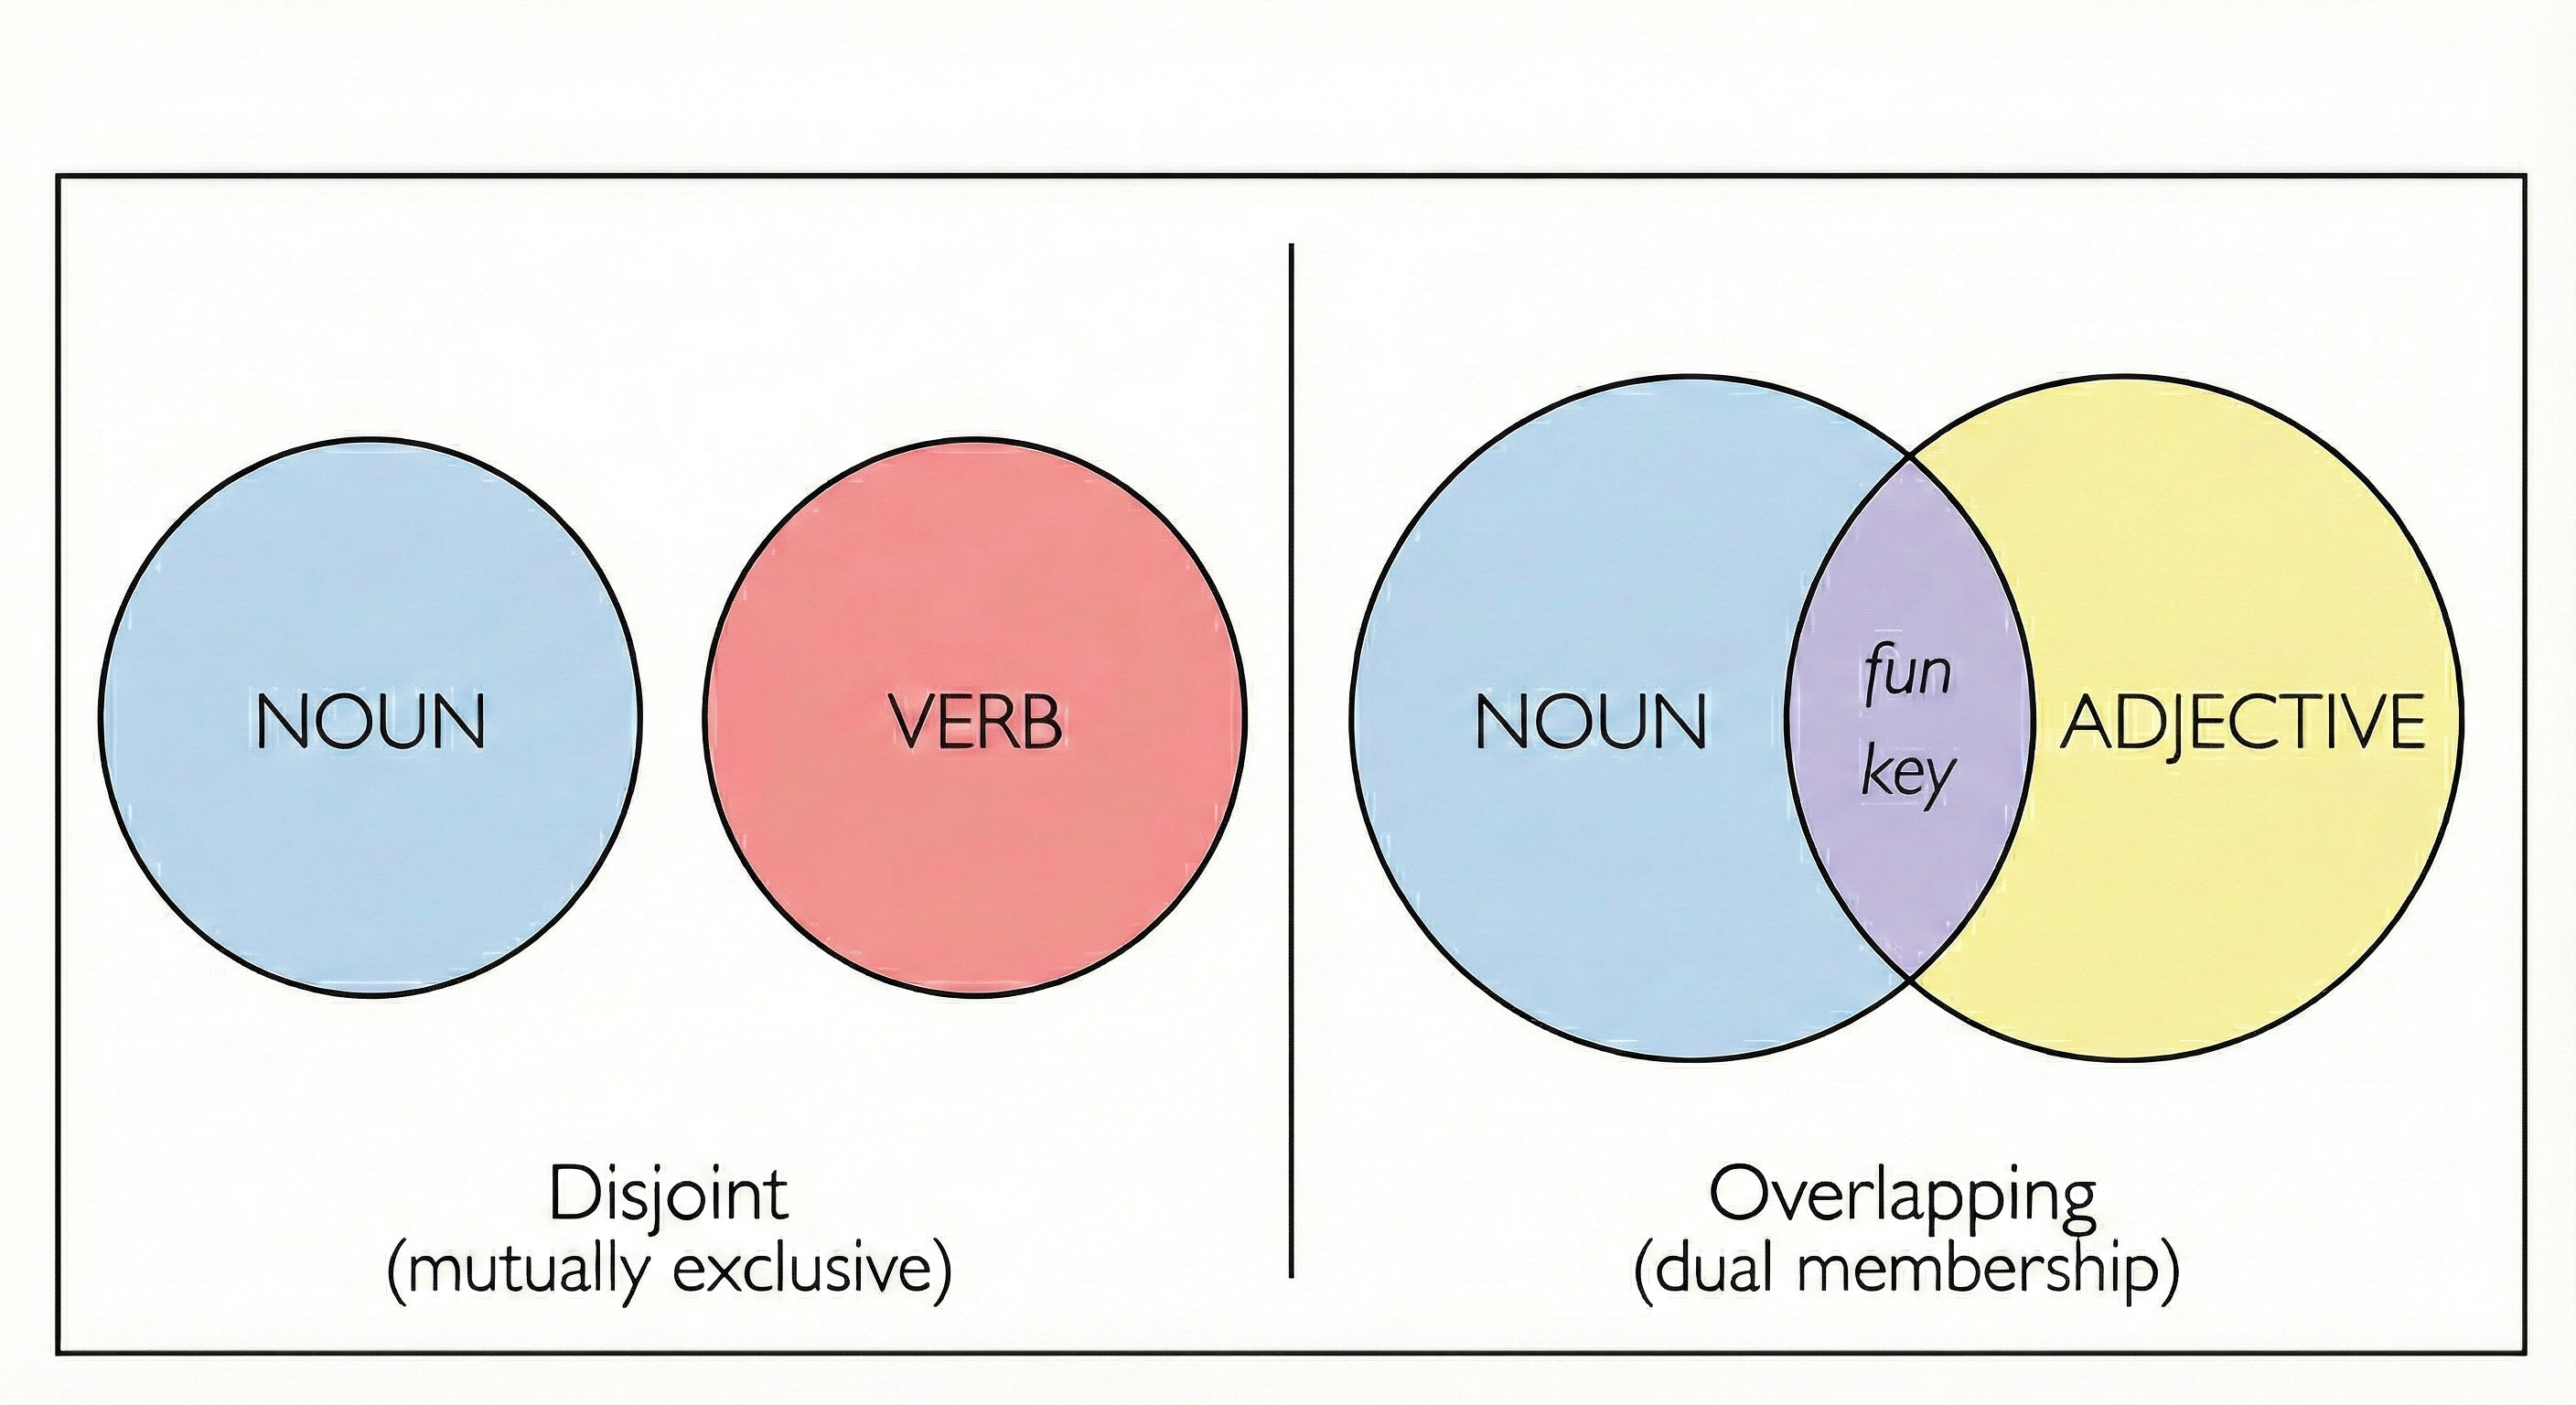
\includegraphics[width=0.85\textwidth]{figures/5.disjoint-overlap.png}
\caption{Disjoint vs.\ overlapping category basins. Left: noun--verb mechanisms pull in opposite directions, creating mutual exclusivity. Right: noun--adjective mechanisms are partially independent, permitting overlap. Items like \mention{fun} and \mention{near} occupy the overlap region, satisfying the clustering criteria for both categories simultaneously.}
\label{fig:disjoint-overlap}
\end{figure}

\subsection{Summary: discreteness without essence}
\label{subsec:5:discreteness-summary}

The discreteness problem asked: if underlying properties are continuous, how do discrete categories emerge?

The answer combines two components:

\textbf{Structure (hyperreal model):} Discrete boundaries arise from scale-dependent tolerance. Changes that are negligible at the current scale preserve categorization; changes that are appreciable can flip it. The boundary is sharp, located at a hyperreal threshold, epistemically inaccessible but structurally determinate. Dynamic discreteness is like a snow-covered streetcar right-of-way: the snowfall is continuous, but the rails impose two stubbornly sharp tracks that exist only because of the system underneath them.

\textbf{Maintenance (HPC framework):} The basin structure persists because mechanisms~-- acquisition, entrenchment, alignment, transmission, functional pressure~-- hold properties together. Without these mechanisms, categories would dissolve. With them, the clustering is stable even though boundaries are fuzzy at the edges.

Together, these explain how categories can be:
\begin{itemize}
\item \textbf{Real}: maintained by causal mechanisms, not merely stipulated.
\item \textbf{Discrete}: with sharp boundaries, not gradient membership.
\item \textbf{Fuzzy at the edges}: because tolerance fails near boundaries, producing instability and apparent gradience.
\item \textbf{Stable}: because mechanisms maintain the basin structure across time.
\item \textbf{Capable of change}: because mechanisms can shift, basins can migrate, boundaries can move.
\end{itemize}

This is what the essentialist wanted~-- real structure, sharp boundaries, determinacy~-- without what the essentialist thought was required: definitions, necessary and sufficient conditions, essences. The categories are real because they're maintained, not because they're defined. The boundaries are sharp because tolerance is scale-dependent, not because some property is binary. The determinacy is causal-structural, not definitional.

The nominalist was right that essences don't exist. The nominalist was wrong to conclude that determinacy fails. The HPC framework, formalised via hyperreal tolerance, shows how to have both: natural kinds without essences, discrete categories from continuous substrates, sharp boundaries that we can't quite see. Dynamic discreteness and real gradience~-- the chapter's twin themes~-- turn out to be two sides of one insight.
